\documentclass[onecolumn, draftclsnofoot,10pt, compsoc]{IEEEtran}
\usepackage{graphicx}
\usepackage{url}
\usepackage{setspace}
\usepackage{graphicx}
\graphicspath{ {./Images/} }

\usepackage{geometry}
\geometry{textheight=9.5in, textwidth=7in}

% 1. Fill in these details
\def \CapstoneTeamName{Proprietors of the Press}
\def \CapstoneTeamNumber{62}
\def \GroupMemberOne{Kuan-Yu Lai}
\def \GroupMemberTwo{Cole Jones}
\def \CapstoneProjectName{Automate the Settings that Control a Million-Dollar Printing Press}
\def \CapstoneSponsorCompany{HP, Inc}
\def \CapstoneSponsorPerson{Pieter van Zee}

% 2. Uncomment the appropriate line below so that the document type works
\def \DocType{		Requirement Document
				%Requirements Document
				%Technology Review
				%Design Document
				%Progress Report
				}
			
\newcommand{\NameSigPair}[1]{\par
\makebox[2.75in][r]{#1} \hfil 	\makebox[3.25in]{\makebox[2.25in]{\hrulefill} \hfill		\makebox[.75in]{\hrulefill}}
\par\vspace{-12pt} \textit{\tiny\noindent
\makebox[2.75in]{} \hfil		\makebox[3.25in]{\makebox[2.25in][r]{Signature} \hfill	\makebox[.75in][r]{Date}}}}
% 3. If the document is not to be signed, uncomment the RENEWcommand below
%\renewcommand{\NameSigPair}[1]{#1}

%%%%%%%%%%%%%%%%%%%%%%%%%%%%%%%%%%%%%%%
\begin{document}
\begin{titlepage}
    \pagenumbering{gobble}
    \begin{singlespace}
        \hfill 
        % 4. If you have a logo, use this includegraphics command to put it on the coversheet.
        %\includegraphics[height=4cm]{CompanyLogo}   
        \par\vspace{.2in}
        \centering
        \scshape{
            \huge CS Capstone \DocType \par
            \large October 25, 2019\par
            \vspace{.75in}
            \textbf{\Huge\CapstoneProjectName\par}\par
            \vspace{1.0in}
            {\large Prepared for}\par
            \Huge \CapstoneSponsorCompany\par
            \vspace{5pt}

            {\Large{\CapstoneSponsorPerson}\par}
            \bigskip
            {\large Prepared by }\par
            Group\CapstoneTeamNumber\par
            % 5. comment out the line below this one if you do not wish to name your team
            \CapstoneTeamName\par 
            \vspace{5pt}
            {\Large
                {\GroupMemberOne}\par
                {\GroupMemberTwo}\par
                {\GroupMemberThree}\par
            }
            \vspace{20pt}
        }
        \vspace{1.0in}
        \begin{abstract}
        % 6. Fill in your abstract    
       	This document describes the details of the automated setting select project that will control the million-dollar presses from HP. It contains subjects like timeline throughout the term, use cases, etc… The main purpose of this document is for people to know what happened during the development process and give the general idea of the final product.
        \end{abstract}     
    \end{singlespace}
\end{titlepage}
\newpage
\pagenumbering{arabic}
\tableofcontents
% 7. uncomment this (if applicable). Consider adding a page break.
\bigskip
\listoffigures

%\listoftables
\clearpage

% 8. now you write!
\section{Overview}
The objective of this project is to create a decision-making engine that takes an input of information about the PDF file to be printed and a data file with additional information about the job (like paper type, color profile, etc.), and outputs a selection of settings used to control the printing press. The engine will run alongside pre-existing internal tools to analyze print jobs within a queue and generate a settings profile (or choose a pre-existing settings profile) for each job on its way out of the queue into the printing press. Once the printing job has reached the printing press, it will display to the operator the settings it has generated, along with a justification as to why that setting was picked and if it aligned with the settings that were chosen or imported. The overall goal is to streamline the processing of picking the correct settings for a print job, reducing the amount of interaction between the operator and the printing press.

\bigskip
\section{Glossary of Terms}
\begin{center}
\begin{tabular}{|c|c|}
  \hline
  \textbf{Term} & \textbf{Description}\\
  \hline
  Ruleset  & A set of rules which the decision-making engine uses to generate optimal job settings.\\ & Includes information about best practices, optimal ink coverage\\ 
  \hline
  Decision-Making Engine   & An engine that allows developers build and run machine reasoning models\\
  \hline
  GUI & Graphical User Interface. The web application used to interact with the engine\\
  \hline
  API & A protocol that allows client communicate with the server easily\\
  \hline
\end{tabular}
\end{center}

\bigskip
\section{Use Cases}
% Saving this just in case it's needed later
%\subsection{Press Operator Interaction}
%\textbf{Scenario:} The operator stands in front of the press and checks if the setting of the %individual task has to be adjusted.\newline
%\textbf{How:} There will be simple signal, possibly checkmark for good and X for unsuitable, %appearing next to each individual setting for the print job. It will suggest to the operator if the %setting has to be changed or not.\newline
%\textbf{Tool:} Machine-learning engine, API linked to the engine.\newline
%\textbf{Success:} The task prints out in excellent quality because of the setting.
\subsection{Implementation of Decision-Making Engine}
\textbf{Scenario:} A decision-making engine will be implemented. This engine will take a set of inputs and produce a set of press settings to append to a print job.\\
\textbf{How:} A collection of candidate engines will be selected through interviews with machine-reasoning experts at OSU in addition to independent research. These decision-making engines will have multiple representative rulesets implemented for testing. Once the engine most suited to the task is found, it will be used to create the final implementation.\\
\textbf{Success:} The final implementation of the engine will be chosen. It will have, in addition to a GUI, an API framework that can be used to communicate with the engine outside of the application. 

\subsection{Use of Decision-Making Engine in Pre-Press Check}
\textbf{Scenario:} The decision-making engine will be used to check if the settings chosen for a job are appropriate.\\
\textbf{How:} This use of the engine will be part of the pre-press check, a check that occurs before a job is queued to make sure it is fit for printing. The engine will analyze the info about the PDF and applied settings and determine whether or not the job should be printed, and if the chosen settings are appropriate or not.\\
\textbf{Success:} The job is checked and a justification for why the settings are appropriate or not is produced. The job will not be sent to a queue.

\subsection{Use of Decision-Making Engine to Generate Job Settings for Job Ticket}
\textbf{Scenario:} The decision-making engine is used to generate optimal job settings from the provided job information. A list of all processed jobs and their outputs is available to the user.\\
\textbf{How:} The engine is used to process multiple jobs and provide an output that consists of a collection of jobs settings stored in a job ticket in addition to justifications as to why those settings were chosen. The engine is not hooked up to a queue. Instead, the user is able to view a list of completed jobs and their outputs, and can take the generated job settings and save them for later use.\\
\textbf{Success:} The user will be able to save created optimal job settings in a database, then use them in later jobs that have similar inputs.

\subsection{Use of Decision-Displaying Current Operating Task and Progress }
\textbf{Scenario:} When the user decides to process their task, they will submit the job ticket so the system can schedule the operation.\\
\textbf{How:} User submits their job ticket, the ticket will be put in the task queue and wait for the press to process the task.\\
\textbf{Success:} The user will be able to see all the tasks, job ticket, in task queue and view the status of each tasks.

\subsection{Use of GUI to Queue Jobs}
\textbf{Scenario:} User has access to a responsive web-based application and make the printing request for the press.\newline
\textbf{How:} The web-based application will have 3 functions: job acquisition, job processing, and job results. Job acquisition only gets the input from the user, the PDF info and job ticket data. The job processing function allows the user to choose some of the printing settings or a settings profile. The settings are different from those that the operator sees, it will be slightly more complicated, with additional information to select rules that the decision-making engine will use. The job results present the current working process of each task and the failure reason if the task failed. Also, it provides a justification for the setting, explaining if the chosen setting matches the setting generated by the decision-making engine or not. \newline
%\textbf{Tool:} React, Hotfolder, API linked to the engine. \newline
\textbf{Success:} Different users will be able to access the same web-based application to queue up jobs or view the queue. The user will not require press operation expertise due to the user-friendly UI.

% Optional use case 
\iffalse 
\subsection{Use of Hotfolder to Queue Jobs}
\textbf{Scenario:} User can place PDF/XML files in a hotfolder to queue it as a print job.\\
\textbf{How:} Users will have access to a hotfolder where they can place documents related to a printing job. A script will detect that new files have been added to the folder and queue them up in for processing by the decision-making engine. The engine will then process the files and add them to the print job queue.\\
\textbf{Success:} The files have been moved from the hotfolder through the decision-making engine and out into the print job queue with appropriate settings attached.
\fi


\subsection{Use of API Calls to Queue Jobs}
\textbf{Scenario:} User can directly call the decision-making engine's API to post PDF info and job ticket data to create a print job.\\
\textbf{How:} A user will use the decision-making engine's built-in API to make a POST call, providing documents relevant to the print job. Similarly to how the hotfolder works, the engine then takes the provided files as input, generate the appropriate settings, and move the job into the print job queue.\\
\textbf{Success:} The files have successfully been processed by the engine and placed into the print job queue with relevant settings information attached.

\pagebreak

\subsection{Selection of Rules for Engine}
\textbf{Scenario:} A user will be able to specify which ruleset the decision-making engine uses for a particular print job.\\
\textbf{How:} During the use of the GUI to select appropriate settings for the print job, the user may specify what ruleset the decision-making engine will use. Each ruleset is like a profile that's adapted to fit certain constraints better, such as the type of paper or the printing press being used.\\
\textbf{Success:} The settings created for a print job will be better-suited for the type of paper and press being used depending on the ruleset used.

% Tools / applications being used
\section{Tools \& Applications}
\subsection{Existing Internal Tool}
There exists an internal tool within HP that allows users to import a PDF of what they want to be printed and XML file that contains some rules about the print job (such as width, paper type, etc.). The user can then select a myriad of settings that the printing press will use to print the job. We will be piggybacking on this tool, inserting our decision-making engine into the pipeline between this internal tool and the print job queue.

\subsection{Decision-Making Engine}
Our decision-making engine will take the settings chosen from the internal tool (or from an XML file) in addition to the PDF of what to print and generate what it determines to be optimal settings for the job. The settings it chooses are based on its analysis of the PDF info and job ticket data. It analyses the size of the document, the density of ink per page, the use of gradients, color fills, and graphics, and determines the optimal printing speed, press tension, and drying heat/time. It will attach the generated settings to the print job when it adds it to the queue, in addition to supplying a justification for each setting choice and a log file to analysis.

\subsection{GUI}
The GUI will be created for user-friendly interaction with the decision-making engine. It will take a PDF info and job ticket data as input. The site will allow the user to drag and drop files into a web interface. It will also allow users to select which ruleset they want the engine to use.

\subsection{API}
An API will be created for the engine to permit its use without having to interact with the GUI. It will be necessary for other applications to provide input without human interference, permitting the engine to run alongside existing programs in the job creation pipeline.

\subsection{Database}
An external database will exist to hold all of the generated rulesets that the engine will use. It will also hold engine output that is deemed reusable for jobs with similar inputs.

%\subsection{Hotfolder}
%The hotfolder will be directly connected to the decision-making engine through its built-in API. When a user places a PDF (and possibly XML) file into the hotfolder, a script will make a POST request to the engine, and the engine will begin processing the job and creating optimal settings. The engine will then place the print job and attached settings into the print job queue.


% Gantt Chart
\pagebreak
\section{Gantt Chart}
\begin{figure}[h]
    \makebox[\textwidth][c]{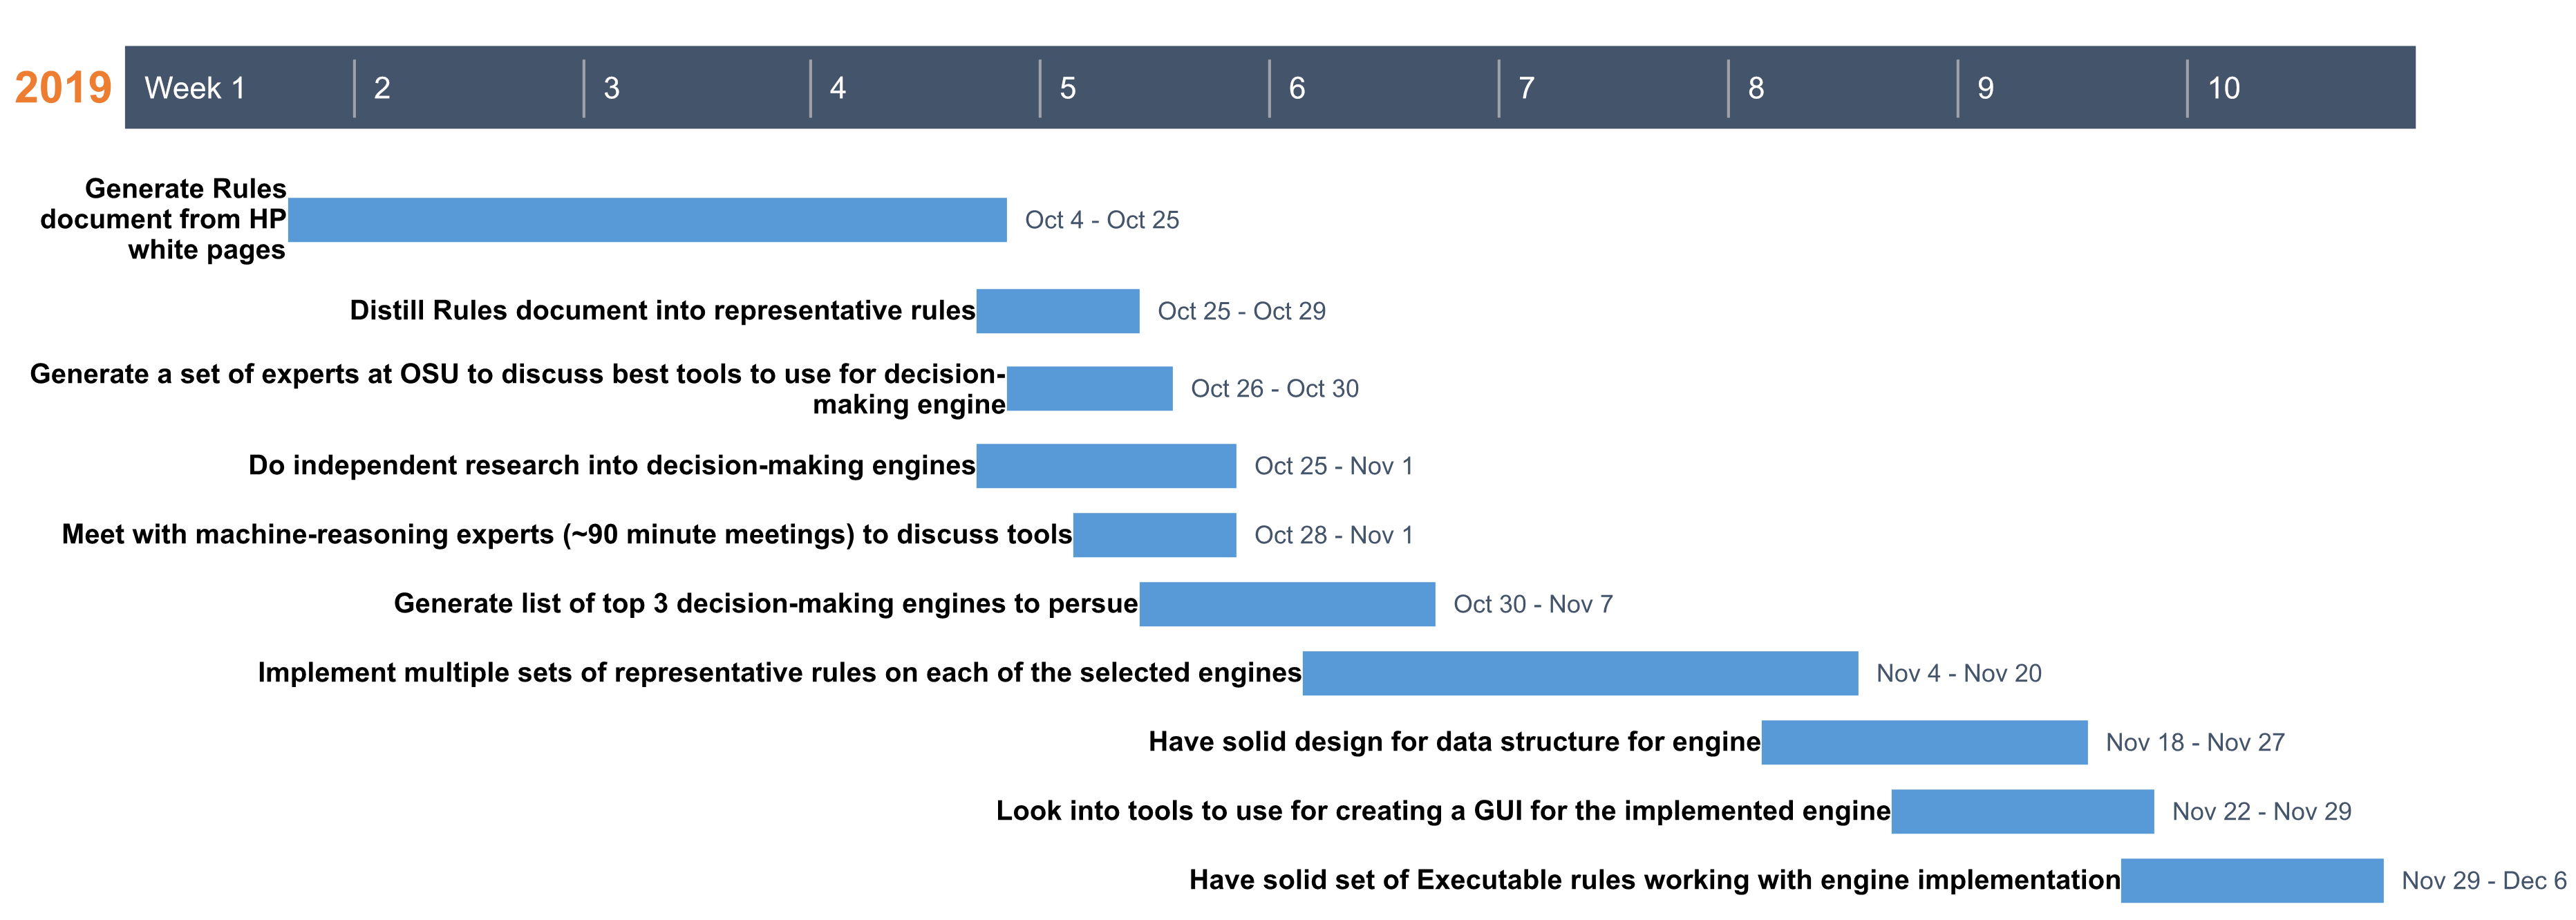
\includegraphics[width=1.05\textwidth]{Gantt}}
    \caption{Gantt Chart}
    \label{fig:1}
\end{figure}

\end{document}